\documentclass[12pt]{article}

\usepackage{sbc-template}
\usepackage{graphicx,url}
\usepackage[utf8]{inputenc}
\usepackage[brazil]{babel}
\usepackage{lipsum}
%\usepackage[latin1]{inputenc}  
\usepackage{amsmath}
\usepackage[portuguese,ruled,vlined]{algorithm2e}
%\usepackage[portuguese,ruled,vlined,linesnumbered]{algorithm2e}
\usepackage{blindtext}
\usepackage{xcolor}
\usepackage{caption}
\usepackage{subcaption}
\usepackage{colortbl}
\usepackage{adjustbox}
\usepackage{tikz}
\usepackage{pgf}
\usepackage{multirow}
\usepackage{pgfplots}
\usepackage{amsmath}
     
\sloppy

\title{Componentes Conexos em Processador Multicore}
\author{Patreze A. Chita \inst{1}, Nahri. B. Moreano\inst{1}}
\address{Faculdade de Computação -- Universidade Federal do Mato Grosso do Sul (UFMS) \\ Caixa Postal 549 -- 79.070.900 -- Campo Grande -- MS -- Brazil
\email{patrezechita@gmail.com, nahri@facom.ufms.br}
}

\begin{document} 

\maketitle

\begin{abstract}
  This meta-paper describes the style to be used in articles and short papers
  for SBC conferences. For papers in English, you should add just an abstract
  while for the papers in Portuguese, we also ask for an abstract in
  Portuguese (``resumo''). In both cases, abstracts should not have more than
  10 lines and must be in the first page of the paper.
\end{abstract}
     
\begin{resumo} 
  Este meta-artigo descreve o estilo a ser usado na confecção de artigos e
  resumos de artigos para publicação nos anais das conferências organizadas
  pela SBC. É solicitada a escrita de resumo e abstract apenas para os artigos
  escritos em português. Artigos em inglês deverão apresentar apenas abstract.
  Nos dois casos, o autor deve tomar cuidado para que o resumo (e o abstract)
  não ultrapassem 10 linhas cada, sendo que ambos devem estar na primeira
  página do artigo.
\end{resumo}

\section{Introdução}
{\color{gray}\lipsum[1]}

\section{Algoritmo Sequencial e Paralelo para Componentes Conexos}
{\color{gray}\lipsum[1]}

\subsection{Algoritmo Sequencial Baseado em Busca em Profundidade}

{\color{gray}\lipsum[1]}

\begin{algorithm}[h]
    \DontPrintSemicolon
    \SetArgSty{textnormal}
    \caption{Algoritmo sequencial para componentes conexos}
    \SetKwProg{ComponentesConexos}{ComponentesConexos}{}{}
    \ComponentesConexos{{\normalfont(grafo G = (V, E))}}
	{
        nComponentes $\gets$ 0\;
        \ParaCada{vértice v $\in$ V}
        {
            visitado[v] $\gets$ FALSO\;
        }
        \ParaCada{vértice v $\in$ V}
        {
            \Se{visitado[v] = FALSO}
            {
                \textbf{DFS}(v)\;
                nComponentes $\gets$ nComponentes + 1\;
            }
        }
    }
    \SetKwProg{DFS}{DFS}{}{}
    \DFS{{\normalfont(vértice v)}}
    {
        componente[v] $\gets$ nComponentes\; 
        visitado[v] $\gets$ VERDADEIRO\;
        \ParaCada{vértice u $\in$ Adj[v]}
        {
            \Se{visitado[u] = FALSO}
            {
                \textbf{DFS}(u)\;
            }
        }
    }
\end{algorithm}

\subsection{Algoritmo Paralelo Baseado em Busca em Profundidade e nas Operações Union/Find}

{\color{gray}\lipsum[1]}

\begin{algorithm}[h]
    \DontPrintSemicolon
    \SetArgSty{textnormal}
    \newcommand\mycommfont[1]{\small\ttfamily{#1}}
	\SetCommentSty{mycommfont}
    \caption{Algoritmo paralelo para componentes conexos}
    \SetKwFor{ForPar}{para cada}{fa\c{c}a em paralelo}{fim para cada}
    \SetKwProg{ComponentesConexosPar}{ComponentesConexosParalelo}{}{}
    \ComponentesConexosPar{{\normalfont(grafo G = (V, E))}}
    {
        p $\gets$ número de processadores\;
        %Divide vértices de $V$ em $p$ partes de $\sim|V|/p$ vértices\;
        dividir a matriz de adjacência de G em p partes\;
        atribuir cada parte da divisão a um dos p processadores\;
        %\tcp{Executar DFS em paralelo, gerando p florestas}
        \ForPar{processador $\text{p}_\text{i}$}
        {
            $\text{E}_\text{i} \gets$ arestas da parte da matriz de adjacência atribuída a $\text{p}_\text{i}$\;
            %$\text{G}_\text{i} \gets$ subgrafo de G induzido por $\text{E}_\text{i}$\;
            subgrafo $\text{G}_\text{i}$ = (V, $\text{E}_\text{i}$)\;
            executar \textbf{DFS}($\text{G}_\text{i}$) produzindo floresta $\text{F}_\text{i}$\;
        }

        unir florestas $\text{F}_\text{i}$, par a par, até restar uma única floresta F\;
        
        %\tcp{Para cada árvore $A$ $\in$ $F$, vértices de $A$ estão no mesmo componente}
        %\tcp{todos os vértices de uma mesma árvore de F pertencem ao mesmo componente}
    }
\end{algorithm}

\section{Solução Paralela para Componentes Conexos para Processador Multicore}

{\color{gray}\lipsum[1]}

\begin{algorithm}[h]
    \DontPrintSemicolon
    \SetArgSty{textnormal}
    \newcommand\mycommfont[1]{\small\ttfamily{#1}}
	\SetCommentSty{mycommfont}
    %\SetAlCapNameFnt{\small} %tamanho nome do algoritmo
    \caption{Implementação do algoritmo paralelo para componentes conexos}
    \SetKwProg{ComponentesConexosPar}{ComponentesConexosParalelo}{}{}
    \SetKwFor{ForPar}{para}{fa\c{c}a em paralelo}{fim para cada}
    \ComponentesConexosPar{{\normalfont(grafo G = (V, E))}}
    {
    	\tcp{Dividir os vértices pelas threads}
        nTh $\gets$ número de threads\;
        nVerticesExtra $\gets |\text{V}|$ -- ($\lfloor \frac{|\text{V}|}{\text{nTh}} \rfloor$ $\times$ nTh)\;
        \ForPar{$t \gets 0$ \Ate $nTh-1$}
        {
            \eSe{t $<$ nVerticesExtra}
            {
                vInicial[t] $\gets$ t $\times$ $\lceil\frac{|\text{V}|}{\text{nTh}}\rceil$\;
                vFinal[t] $\gets$ vInicial[t] + $\lceil\frac{|\text{V}|}{\text{nTh}}\rceil$ -- 1\;
            }
           {
                vInicial[t] $\gets$ t $\times$ $\lfloor\frac{|\text{V}|}{\text{nTh}}\rfloor$ + nVerticesExtra\;
                vFinal[t] $\gets$ vIncial[t] + $\lfloor\frac{|\text{V}|}{\text{nTh}}\rfloor$ -- 1\;
            }
        }
        \tcp{Executar DFS em paralelo, gerando nTh florestas}
        \ParaCada{vértice v $\in$ V}
        {
            visitado[v] $\gets$ FALSO\;
        }
        \ForPar{t $\gets$ 0 \Ate nTh -- 1}
        {
            \ParaCada{vértice v $\in$ V}
            {
                componente[t][v] $\gets$ v\;
            }
            floresta[t] $\gets$ \{$\emptyset$\}\;
            \Para{v $\gets$ vInicial[t] \Ate vFinal[t]}
            {
                \Se{visitado[v] = FALSO}
                {
                    raiz $\gets$ v\;
                    \textbf{DFS}(t, v, raiz)\;
                }
            }
        }
        \tcp{Unir pares de florestas em paralelo}
        nPares $\gets \frac{\text{nTh}}{\text{2}}$\;
        \Para{i $\gets$ 0 \Ate $\log_2\!\text{(nTh)}$ -- 1}
        {
            \ForPar{t $\gets$ 0 \Ate nPares -- 1}
            {
                thEsquerda $\gets$ t $\times$ $\text{2}^{\text{i+1}}$\;
                thDireita $\gets$ thEsquerda + $\text{2}^\text{i}$\;
                
                \ParaCada{aresta (v, u) $\in$ floresta[thDireita]}
                {
                    \textbf{Union}(thEsquerda, v, u)\;
                }
            }
            nPares $\gets \frac{\text{nPares}}{\text{2}}$\;
        }
    }
    \SetKwProg{DFS}{DFS}{}{}
    \DFS{{\normalfont(thread t, vértice v, vértice raiz)}}
    {
        componente[t][v] $\gets$ raiz\;
        
        \ParaCada{vértice u $\in$ Adj[v]}
        {
            floresta[t] $\gets$ floresta[t] $\cup$ \{(v, u)\}\;
            componente[t][u] $\gets$ raiz\;
            
            \Se{vInicial[t] $\le$ u \textbf{\upshape e} u $\le$ vFinal[t]}
            {
                \Se{visitado[u] = FALSO}
                {
                    \textbf{DFS}(t, u, raiz)\;
                }
            }
        }
        visitado[v] $\gets$ VERDADEIRO\;
    }
\end{algorithm}
    
\begin{algorithm}[h]
    \DontPrintSemicolon
    \SetArgSty{textnormal}
    \caption{Operações Union e Find}
    \SetKw{Return}{retorna}
    \SetKwProg{UNION}{Union}{}{}
    \UNION{{\normalfont(thread t, vértice v, vértice u)}}
    {
        vComponente $\gets$ \textbf{Find}(t, v)\;
        uComponente $\gets$ \textbf{Find}(t, u)\;
        min $\gets$ \textbf{Mínimo}(vComponente, uComponente)\;
		max $\gets$ \textbf{Máximo}(vComponente, uComponente)\;
        \Se{vComponente $\neq$ uComponente}
        {
            \ParaCada{vértice i $\in$ V}
            {
                \Se{componente[t][i] = max}
                {
                    componente[t][i] $\gets$ min\;
                }
            }
            floresta[t] $\gets$ floresta[t] $\cup$ \{(v, u)\}\;
        }
    }
    \SetKwProg{FIND}{Find}{}{}
    \FIND{{\normalfont(thread t, vértice v)}}
    {
        \Return componente[t][v]\;
    }
\end{algorithm}

\section{Resultados e Análise}

\begin{figure}[h]
    \centering
    \begin{minipage}{.48\textwidth}
        \centering
        \resizebox{\textwidth}{!}
        {
			\begin{tikzpicture}
			\begin{axis}[
				%title={Execução alg par 25k com várias threads},
				legend pos=north west,
				xlabel={quantidade de vértices},
				%legend style={at={(0.5,-0.20)},anchor=north,legend columns=-1},
				%symbolic x coords={a,b,c,d},
				ylabel={tempo de execução (s)},
				xtick=data,
				symbolic x coords={5K, 10K, 15K, 25K}]
				\addplot coordinates {
					(5K,2.9988)(10K,13.7175)(15K,37.0794)(25K,112.2789)};
				\addplot coordinates {
					(5K,1.1584)(10K,4.8591)(15K,12.4221)(25K,37.0791)};
			\legend{Sequencial, Paralelo}
			\end{axis}
			\end{tikzpicture}
		}
        \caption{tempo densid 100\% 8 th}
    \end{minipage}\hfill%
    \begin{minipage}{.48\textwidth}
        \centering
        \resizebox{\textwidth}{!}
        {
			\begin{tikzpicture}
			\begin{axis}[
				%title={Execução alg par 25k com várias threads},
				legend pos=north west,
				xlabel={densidade do grafo},
				%legend style={at={(0.5,-0.20)},anchor=north,legend columns=-1},
				%symbolic x coords={a,b,c,d},
				ylabel={tempo de execução (s)},
				xtick=data,
				symbolic x coords={5\%, 25\%, 50\%, 75\%, 100\%}]
				\addplot coordinates {
					(5\%,4.0333)(25\%,24.6417)(50\%,53.7326)(75\%,82.9658)(100\%,112.2789)};
				\addplot coordinates {
					(5\%,1.6681)(25\%,9.6514)(50\%,19.8564)(75\%,29.1588)(100\%,37.0791)};
			\legend{Sequencial, Paralelo}
			\end{axis}
			\end{tikzpicture}
		}
        \caption{tempo grafo 25K 8th}
    \end{minipage}
\end{figure}

\begin{figure}[h]
    \centering
    \begin{minipage}{.48\textwidth}
        \centering
        \resizebox{\textwidth}{!}
        {
			\begin{tikzpicture}
			\begin{axis}[
				%title={Execução alg par 25k com várias threads},
				legend style={at={(0.5,1.15)},anchor=north,legend columns=-1},
				xlabel={quantidade de vértices},
				%legend style={at={(0.5,-0.20)},anchor=north,legend columns=-1},
				%symbolic x coords={a,b,c,d},
				ylabel={\emph{speedup}},
				xtick=data,
				symbolic x coords={5K, 10K, 15K, 25K}]
				\addplot coordinates {
					(5K,1.96)(10K,2.10)(15K,2.19)(25K,2.42)};
				\addplot coordinates {
					(5K,2.26)(10K,2.50)(15K,2.43)(25K,2.55)};
				\addplot coordinates {
					(5K,2.37)(10K,2.51)(15K,2.54)(25K,2.71)};
				\addplot coordinates {
					(5K,2.54)(10K,2.60)(15K,2.74)(25K,2.85)};
				\addplot coordinates {
					(5K,2.59)(10K,2.82)(15K,2.98)(25K,3.03)};
			\legend{5\%, 25\%, 50\%, 75\%, 100\%}
			\end{axis}
			\end{tikzpicture}
		}
        \caption{speedup dens 8th}
    \end{minipage}\hfill%
    \begin{minipage}{.48\textwidth}
        \centering
        \resizebox{\textwidth}{!}
        {
			\begin{tikzpicture}
			\begin{axis}[
				legend pos=north west,
				%legend style={at={(0.5,1.15)},anchor=north,legend columns=-1},
				%xlabel={densidade do grafo},
				%legend style={at={(0.5,-0.20)},anchor=north,legend columns=-1},
				%symbolic x coords={a,b,c,d},
				ylabel={\emph{speedup}},
				xlabel={densidade do grafo},
				xtick=data,
				symbolic x coords={5\%, 25\%, 50\%, 75\%, 100\%}]
				\addplot coordinates {
					(5\%,1.96)(25\%,2.26)(50\%,2.37)(75\%,2.54)(100\%,2.59)};
				\addplot coordinates {
					(5\%,2.10)(25\%,2.50)(50\%,2.51)(75\%,2.60)(100\%,2.82)};
				\addplot coordinates {
					(5\%,2.19)(25\%,2.43)(50\%,2.54)(75\%,2.74)(100\%,2.98)};
				\addplot coordinates {
					(5\%,2.42)(25\%,2.55)(50\%,2.71)(75\%,2.85)(100\%,3.03)};
			\legend{5K, 10K, 15K, 25K}
			\end{axis}
			\end{tikzpicture}
		}
        \caption{speedup qtd ver 8th}
    \end{minipage}
\end{figure}

\begin{figure}[h]
    \centering
    \begin{minipage}{.48\textwidth}
        \centering
        \resizebox{\textwidth}{!}
        {
			\begin{tikzpicture}
				\begin{axis}
				[
					legend pos=north west,
					%x tick label style={/pgf/number format/1000 sep=},
					ylabel={tempo de execução (s)},
					xlabel={densidade do grafo},
					enlargelimits=0.15,
					ybar,
					nodes near coords,
					nodes near coords align={vertical},
					bar width=17.5pt,
					symbolic x coords={5\%, 25\%, 50\%, 75\%, 100\%},
					]
				]
			\addplot 
				coordinates {(5\%,1.6681)(25\%,9.6514)(50\%,19.8)(75\%,29.1)(100\%,37.1)};
			\legend{25K}
			\end{axis}
			\end{tikzpicture}
		}
        \caption{tempo grafo 25K 8th}
    \end{minipage}\hfill%
    \begin{minipage}{.48\textwidth}
        \centering
        \resizebox{\textwidth}{!}
        {
			\begin{tikzpicture}
			\begin{axis}[
				legend pos=north west,
				xlabel={densidade do grafo},
				%legend style={at={(0.5,-0.20)},anchor=north,legend columns=-1},
				%symbolic x coords={a,b,c,d},
				ylabel={tempo de execução (s)},
				%xtick=data,
				symbolic x coords={5\%, 25\%, 50\%, 75\%, 100\%}]
				\addplot coordinates {
					(5\%,2.9733)(25\%,17.3807)(50\%,36.9300)(75\%,56.7824)(100\%,71.7106)
				};
				\addplot coordinates {
					(5\%,2.0330)(25\%,12.3225)(50\%,26.4038)(75\%,40.3008)(100\%,48.8452)
				};
				\addplot coordinates {
					(5\%,1.6745)(25\%,9.7046)(50\%,19.8150)(75\%,29.0185)(100\%,37.0678)
				};
			\legend{2 $th$,4 $th$,8 $th$}
			\end{axis}
			\end{tikzpicture}
		}
        \caption{tempo 25K varias th}
    \end{minipage}
\end{figure}

{\color{gray}\lipsum[1]}





\section{Conclusão}

{\color{gray}\lipsum[1]}

\begin{figure}[h]
	\centering
	\subcaptionbox{}[.32\textwidth]
	{
		\resizebox{0.3\textwidth}{!}
        {
			\begin{tikzpicture}
			[scale=1,auto=left,every node/.style={circle,fill=gray!20}]
				\node (v0) at (0,4) {0};
				\node (v6) at (0,0) {6};
				\node (v3) at (0,2) {3};
				\node (v2) at (2,4) {2};
				\node (v1) at (6,4) {1};
				\node (v4) at (6,2) {4};
				\node (v5) at (4,2) {5};
				\node (v7) at (6,0) {7};
				\node (v8) at (2,0) {8};
				\node (v9) at (4,0) {9};
				\node [fill=white!0](x) at (0,-1) {}; %vértice invisível para alinhar 
				\foreach \from/\to in {v0/v3,v3/v6,v3/v2,v0/v2,v1/v4,v4/v5,v4/v7,v8/v9}
				\draw[line width=1.5pt] (\from) -- (\to);
			\end{tikzpicture}
		}
	}
	\subcaptionbox{}[.32\textwidth]
	{
		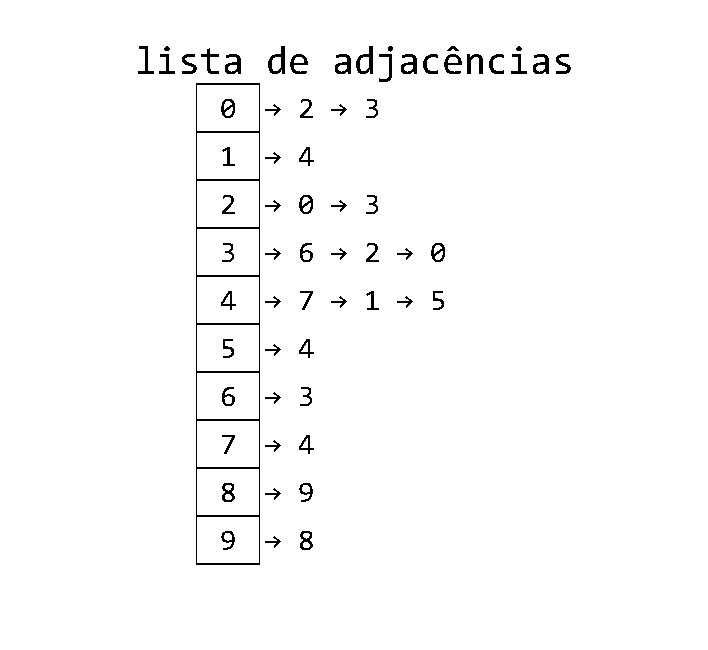
\includegraphics[width=\linewidth]{figB.pdf}
	}
	\subcaptionbox{}[.32\textwidth]
	{
		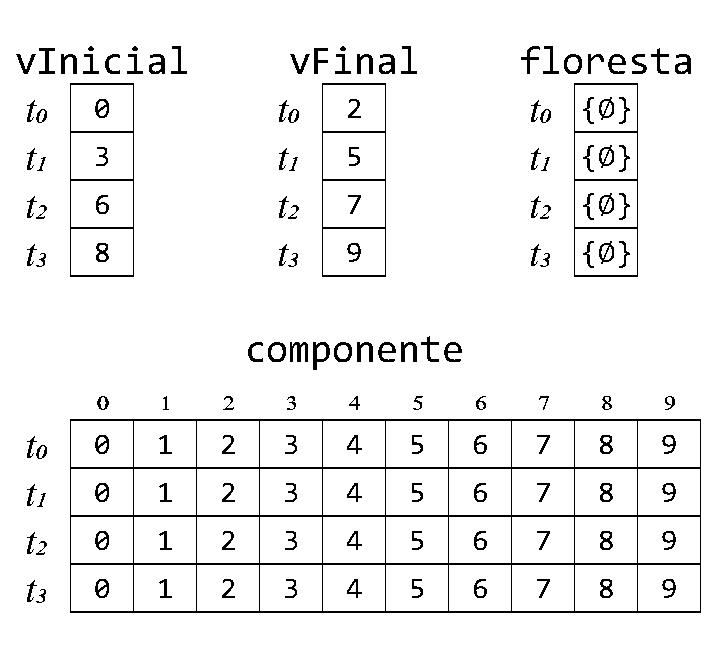
\includegraphics[width=\linewidth]{figC.pdf}
	}
	\subcaptionbox{}[.32\textwidth]
	{
		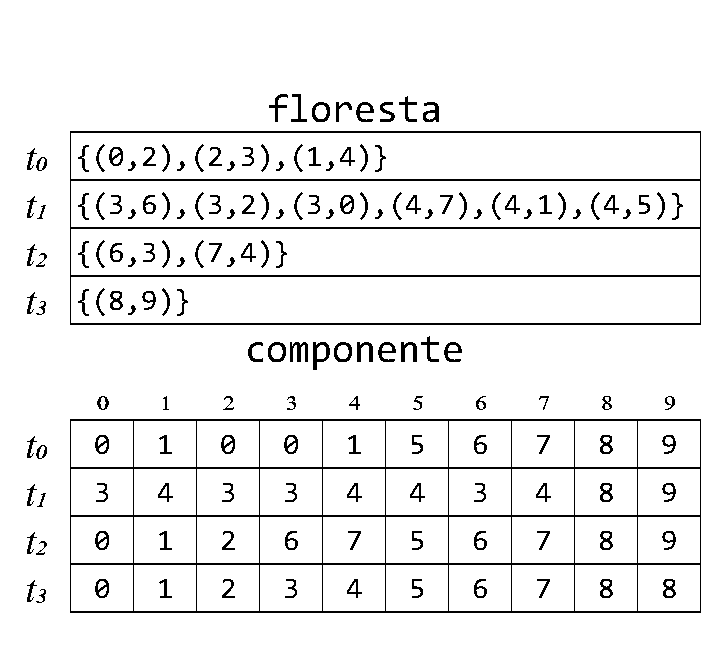
\includegraphics[width=\linewidth]{figD.pdf}
	}
	\subcaptionbox{}[.32\textwidth]
	{
		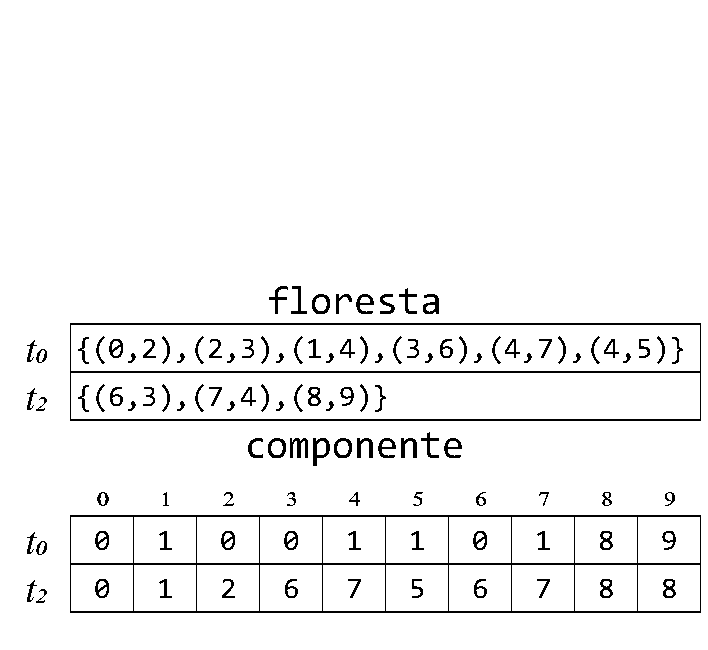
\includegraphics[width=\linewidth]{figE.pdf}
	}
	\subcaptionbox{}[.32\textwidth]
	{
		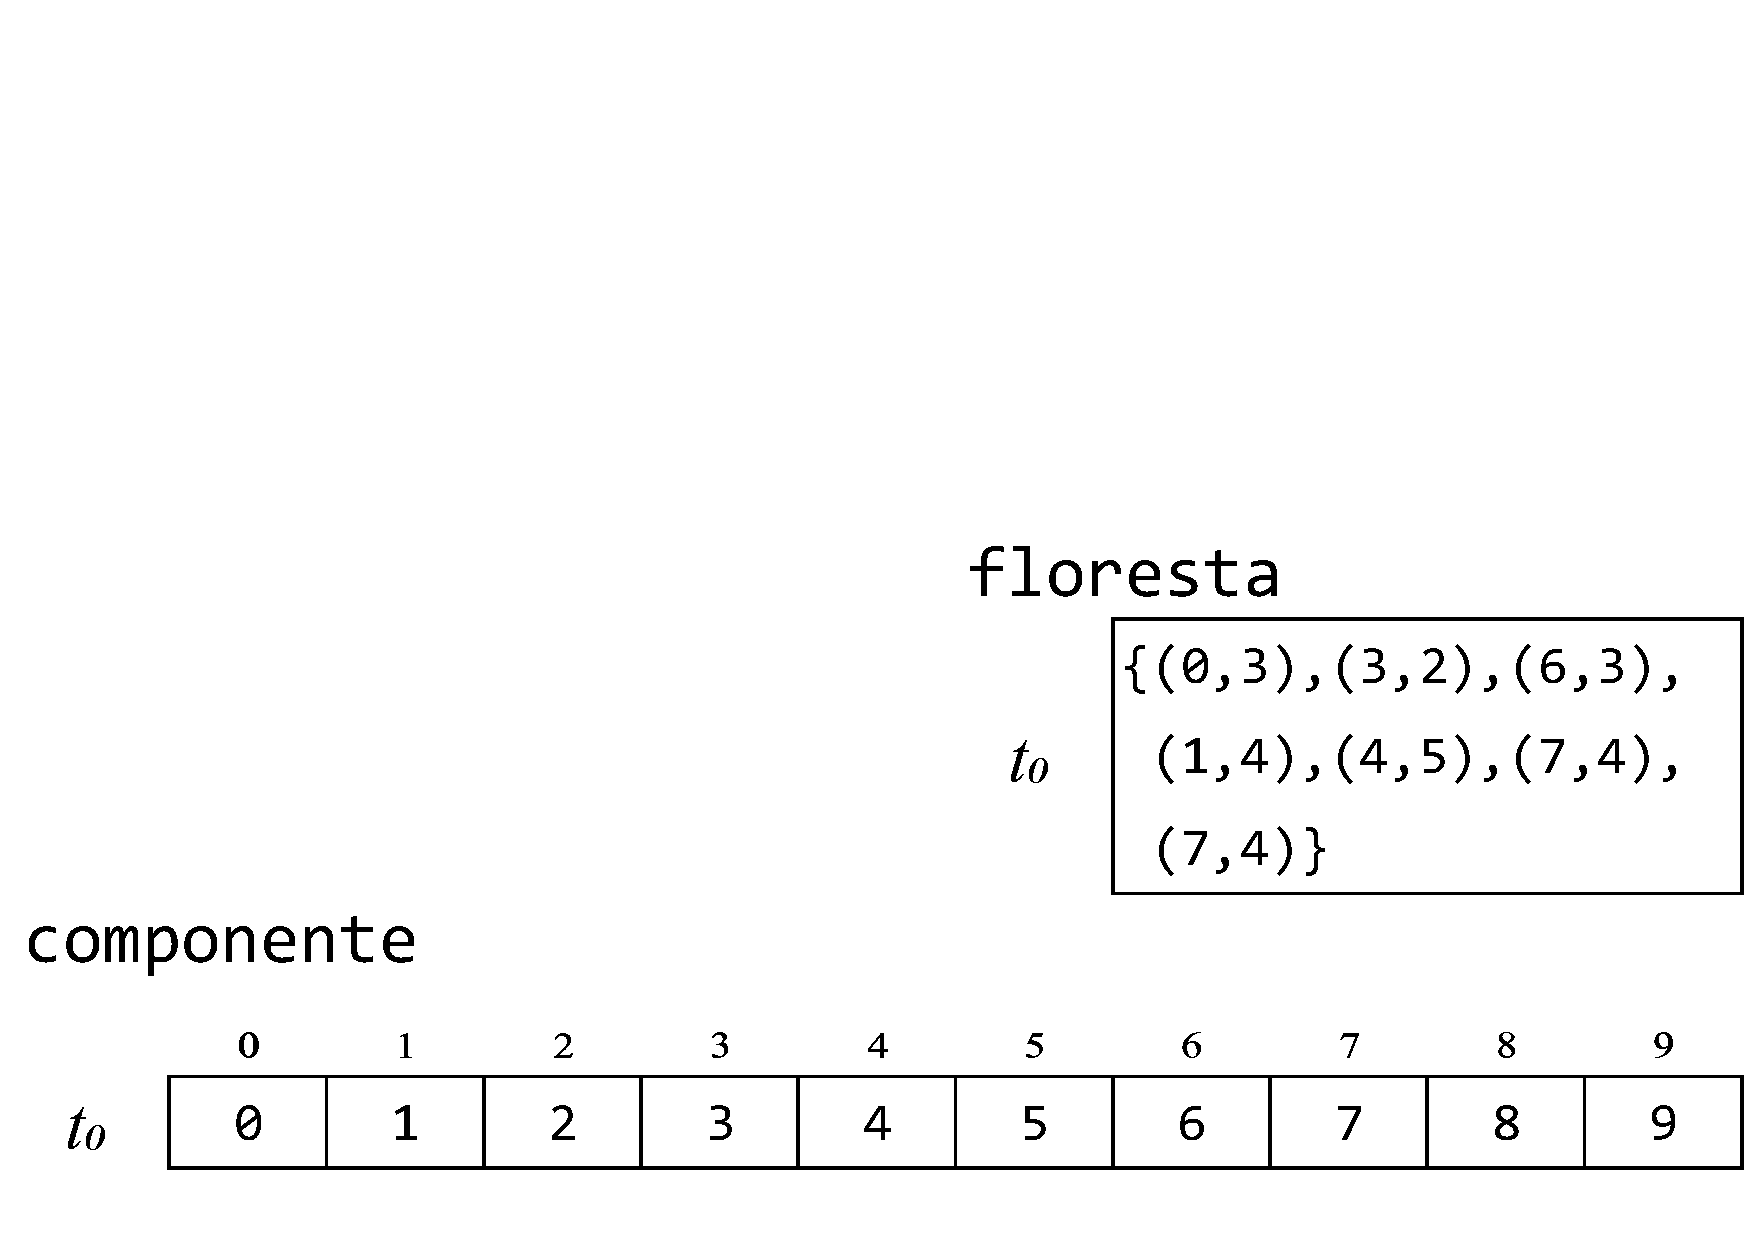
\includegraphics[width=\linewidth]{figF.pdf}
	}
	\caption{Execução da implementação do algoritmo paralelo. (a) Representação gráfica de G=(V, E). (b) A lista de adjacências do grafo G. (c) Estado das estruturas antes de iniciar o DFS paralelo. (d) Estado das estruturas após terminar de executar o DFS em paralelo. (e) Estado das estruturas após fazer a primeira rodada de uniões em paralelo. (f) Estado das estruturas após fazer a segunda rodada de uniões, sendo que a \emph{thread} 0 possui o resultado do algoritmo.}
\end{figure}

\bibliographystyle{sbc}
\bibliography{sbc-template}

\end{document}
